\documentclass[12pt,a4paper]{article}
\usepackage{amsmath, amssymb, amsthm}
\usepackage[utf8]{inputenc}
\usepackage[T1]{fontenc}
\usepackage{geometry}
\usepackage{tikz}
\usetikzlibrary{arrows.meta, calc, 3d, perspective, decorations.pathmorphing, shapes, positioning}
\geometry{margin=2.5cm}

\newtheorem{definition}{Definition}
\newtheorem{theorem}{Theorem}
\newtheorem{example}{Example}
\newtheorem{remark}{Remark}

\title{Infinitesimal Calculus 2 --- Lecture 4 (18.03.2026)\\
\large Differentiability and Partial Derivatives}
\date{}

\begin{document}
\maketitle

%----------------------------------------------------------
\section*{Partial Derivatives --- Formal Definitions}
%----------------------------------------------------------

For $z = f(x,y)$ at $(x_0,y_0)$, the increments are:
\[
  \Delta_x f(x_0,y_0) = f(x_0+\Delta x,\,y_0) - f(x_0,y_0),\qquad
  \Delta_y f(x_0,y_0) = f(x_0,\,y_0+\Delta y) - f(x_0,y_0).
\]

\begin{definition}[Partial derivatives]
\begin{align*}
  f'_x(x_0,y_0) &= \lim_{\Delta x\to 0}\frac{\Delta_x f(x_0,y_0)}{\Delta x}
    = \lim_{\Delta x\to 0}\frac{f(x_0+\Delta x,\,y_0)-f(x_0,y_0)}{\Delta x},\\[6pt]
  f'_y(x_0,y_0) &= \lim_{\Delta y\to 0}\frac{\Delta_y f(x_0,y_0)}{\Delta y}
    = \lim_{\Delta y\to 0}\frac{f(x_0,\,y_0+\Delta y)-f(x_0,y_0)}{\Delta y}.
\end{align*}
\end{definition}

\subsubsection*{Geometric meaning of partial derivatives}

\begin{center}
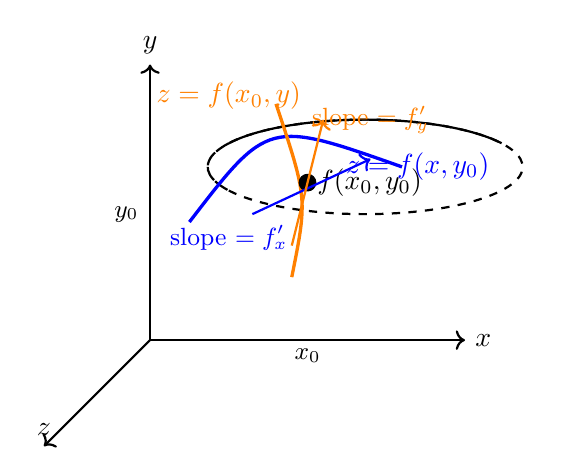
\begin{tikzpicture}[scale=1.0]
  % Draw a surface-like shape (ellipse top view perspective)
  % axes
  \draw[->, thick] (0,0,0) -- (4,0,0) node[right] {$x$};
  \draw[->, thick] (0,0,0) -- (0,3.5,0) node[above] {$y$};
  \draw[->, thick] (0,0,0) -- (0,0,3.5) node[above] {$z$};

  % Surface outline (drawn as a skewed ellipse to simulate 3D)
  \draw[thick] (1.0,2.5) arc[start angle=150, end angle=30, x radius=2.0, y radius=0.6];
  \draw[thick, dashed] (1.0,2.5) arc[start angle=150, end angle=210+360, x radius=2.0, y radius=0.6];

  % Cross-section z = f(x, y0) -- curve in x direction (blue)
  \draw[blue, very thick] (0.5,1.5) .. controls (1.5,2.8) .. (3.2,2.2);
  \node[blue] at (3.4,2.2) {$z=f(x,y_0)$};

  % Cross-section z = f(x0, y) -- curve in y direction (orange)
  \draw[orange, very thick] (1.8,0.8) .. controls (2.0,1.8) .. (1.6,3.0);
  \node[orange] at (1.0,3.1) {$z=f(x_0,y)$};

  % Point on surface
  \filldraw[black] (2.0,2.0) circle (3pt) node[right] {$f(x_0,y_0)$};

  % tangent lines at the point
  \draw[blue, thick, ->] (1.3,1.6) -- (2.8,2.3);
  \node[blue] at (1.0,1.3) {\small slope $= f'_x$};
  \draw[orange, thick, ->] (1.8,1.2) -- (2.2,2.8);
  \node[orange] at (2.8,2.8) {\small slope $= f'_y$};

  % x0, y0 labels
  \node at (2.0,-0.2) {\small $x_0$};
  \node at (-0.3,1.6) {\small $y_0$};
\end{tikzpicture}
\end{center}

$f'_x(x_0,y_0)$ is the slope of the cross-section $z=f(x,y_0)$ (blue curve) at $x_0$.\\
$f'_y(x_0,y_0)$ is the slope of the cross-section $z=f(x_0,y)$ (orange curve) at $y_0$.

%----------------------------------------------------------
\section*{Differentiability}
%----------------------------------------------------------

\begin{definition}[Differentiable function]
$z=f(x,y)$ is \textbf{differentiable} at $(x_0,y_0)$ if:
\[
  \Delta f(x_0,y_0) = A\,\Delta x + B\,\Delta y + \alpha\,\Delta x + \beta\,\Delta y,
  \qquad \alpha,\beta\to 0 \;\text{as}\; \Delta x,\Delta y\to 0.
\]
The \textbf{total differential} is $df(x_0,y_0) = A\,\Delta x + B\,\Delta y$.
\end{definition}

Setting $\Delta\rho = \sqrt{(\Delta x)^2+(\Delta y)^2}$ and writing $\varepsilon\cdot\Delta\rho = \alpha\,\Delta x+\beta\,\Delta y$:
\[
  \varepsilon = \alpha\cdot\underbrace{\tfrac{\Delta x}{\Delta\rho}}_{\cos\theta}
              + \beta\cdot\underbrace{\tfrac{\Delta y}{\Delta\rho}}_{\sin\theta} \to 0
  \quad\text{as }\Delta\rho\to 0.
\]

%----------------------------------------------------------
\section*{Main Theorems}
%----------------------------------------------------------

\begin{theorem}[Thm 1: Differentiable $\Rightarrow$ Continuous]
If $f$ is differentiable at $(x_0,y_0)$, then $f$ is continuous there.

\textit{Proof}: $\Delta f = A\,\Delta x+B\,\Delta y+\alpha\,\Delta x+\beta\,\Delta y\to 0$.
\end{theorem}

\begin{theorem}[Thm 2: Differentiable $\Rightarrow$ Partial derivatives exist; $A=f'_x$, $B=f'_y$]
Set $\Delta y=0$: $\;\Delta_x f = (A+\alpha)\,\Delta x$. Dividing by $\Delta x$ and taking the limit gives $f'_x = A$. Similarly $f'_y = B$.
\end{theorem}

\begin{theorem}[Thm 3: Continuous partials $\Rightarrow$ Differentiable]
If $f'_x,f'_y$ exist and are continuous at $(x_0,y_0)$, then $f$ is differentiable there.

\textit{Proof sketch (Lagrange MVT)}:
\begin{align*}
  \Delta f &= \underbrace{f(x_0+\Delta x,y_0+\Delta y)-f(x_0,y_0+\Delta y)}_{\text{MVT on }x}
           + \underbrace{f(x_0,y_0+\Delta y)-f(x_0,y_0)}_{\text{MVT on }y} \\
  &= f'_x(\tilde{x},y_0+\Delta y)\,\Delta x + f'_y(x_0,\tilde{y})\,\Delta y \\
  &= \bigl(f'_x(x_0,y_0)+\alpha\bigr)\Delta x + \bigl(f'_y(x_0,y_0)+\beta\bigr)\Delta y,
  \quad \alpha,\beta\to 0.
\end{align*}

\begin{center}
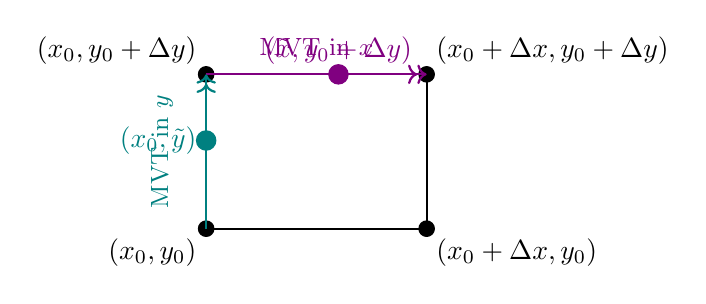
\begin{tikzpicture}[scale=1.4]
  % Rectangle for MVT proof
  \draw[thick] (0,0) rectangle (2.0,1.4);
  % corners
  \filldraw (0,0) circle (2pt) node[below left] {$(x_0,y_0)$};
  \filldraw (2.0,0) circle (2pt) node[below right] {$(x_0+\Delta x,y_0)$};
  \filldraw (0,1.4) circle (2pt) node[above left] {$(x_0,y_0+\Delta y)$};
  \filldraw (2.0,1.4) circle (2pt) node[above right] {$(x_0+\Delta x,y_0+\Delta y)$};
  % intermediate points
  \filldraw[violet] (1.2,1.4) circle (2.5pt) node[above] {$(\tilde{x},y_0+\Delta y)$};
  \filldraw[teal] (0,0.8) circle (2.5pt) node[left] {$(x_0,\tilde{y})$};
  % horizontal MVT arrow
  \draw[violet, ->>, thick] (0,1.4) -- (2.0,1.4);
  \node[violet] at (1.0,1.65) {\small MVT in $x$};
  % vertical MVT arrow
  \draw[teal, ->>, thick] (0,0) -- (0,1.4);
  \node[teal, rotate=90] at (-0.4,0.7) {\small MVT in $y$};
\end{tikzpicture}
\end{center}
\end{theorem}

\subsection*{Hierarchy of Properties}

\begin{center}
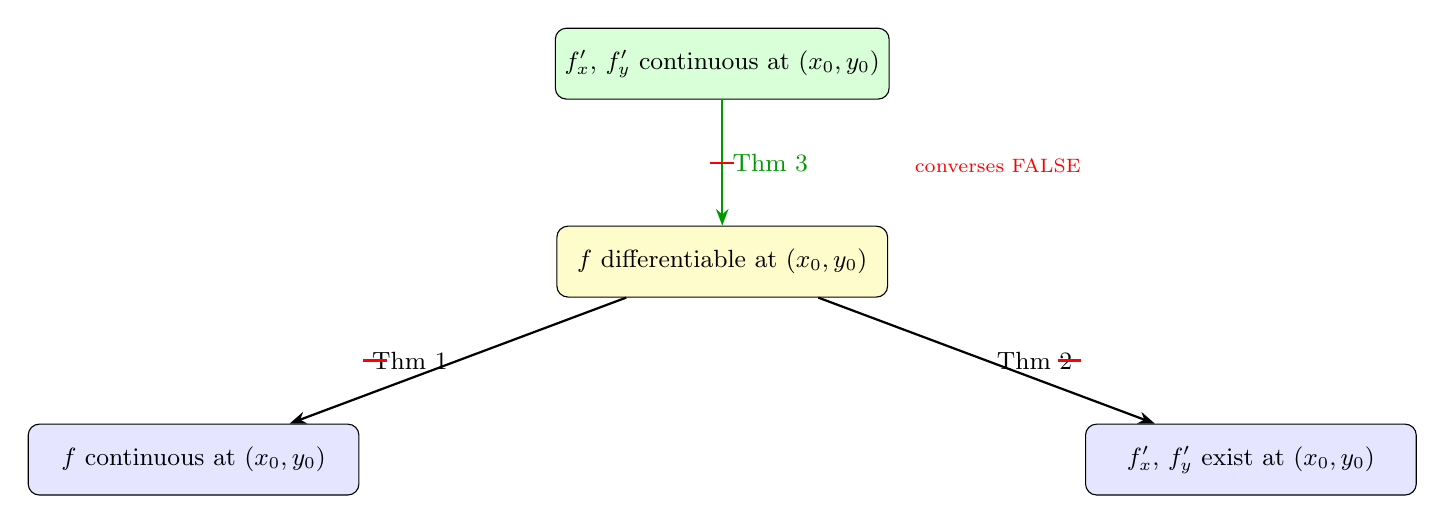
\begin{tikzpicture}[
  node distance=1.6cm and 2.5cm,
  box/.style={draw, rounded corners, minimum width=4.2cm, minimum height=0.9cm,
              text centered, font=\small},
  arr/.style={-{Stealth[length=6pt]}, thick}
]
  \node[box, fill=green!15] (A) {$f'_x,\,f'_y$ continuous at $(x_0,y_0)$};
  \node[box, fill=yellow!20, below=of A] (B) {$f$ differentiable at $(x_0,y_0)$};
  \node[box, fill=blue!10, below left=of B] (C) {$f$ continuous at $(x_0,y_0)$};
  \node[box, fill=blue!10, below right=of B] (D) {$f'_x,\,f'_y$ exist at $(x_0,y_0)$};

  \draw[arr, green!60!black] (A) -- (B) node[midway, right] {\small Thm 3};
  \draw[arr] (B) -- (C) node[midway, left] {\small Thm 1};
  \draw[arr] (B) -- (D) node[midway, right] {\small Thm 2};

  % crossed converses
  \draw[red, thick] ($(C.north)!0.5!(B.south west)$) +(-0.15,0) -- +(0.15,0);
  \draw[red, thick] ($(D.north)!0.5!(B.south east)$) +(-0.15,0) -- +(0.15,0);
  \draw[red, thick] ($(B.north)!0.5!(A.south)$) +(-0.15,0) -- +(0.15,0);

  \node[red, font=\scriptsize] at (3.5,-1.3) {converses FALSE};
\end{tikzpicture}
\end{center}

%----------------------------------------------------------
\section*{Examples}
%----------------------------------------------------------

\begin{example}[Differentiable --- check from definition]
$f(x,y)=x^2-xy$ at $(1,4)$.
\begin{align*}
  \Delta f(1,4) &= (1+\Delta x)^2-(1+\Delta x)(4+\Delta y)-[1-4]\\
  &= -2\Delta x - \Delta y
     + \underbrace{(\Delta x)^2}_{\alpha=\Delta x}
     - \underbrace{\Delta x\,\Delta y}_{\beta=-\Delta y}.
\end{align*}
So $f$ is differentiable at $(1,4)$ and $df(1,4) = -2\,\Delta x - \Delta y$.

Check: $f'_x = 2x-y \Rightarrow f'_x(1,4)=-2$; $\;f'_y=-x \Rightarrow f'_y(1,4)=-1$. \checkmark
\end{example}

\begin{example}[Partial derivatives exist, NOT continuous, NOT differentiable]
\[
  f(x,y)=\begin{cases}\dfrac{xy}{x^2+y^2},&(x,y)\ne(0,0),\\0,&(x,y)=(0,0).\end{cases}
\]
$f'_x(0,0)=\lim_{\Delta x\to 0}\frac{\Delta x\cdot 0/(\Delta x)^2-0}{\Delta x}=0$,
similarly $f'_y(0,0)=0$.

But along $x=y\to 0$: $f\to\frac{1}{2}\ne 0$. So $f$ is \textbf{not continuous}, hence
\textbf{not differentiable} at $(0,0)$.
\end{example}

\begin{example}[Continuous but NO partial derivatives]
\[
  f(x,y)=|x|+\sqrt[3]{y^2}.
\]

\begin{center}
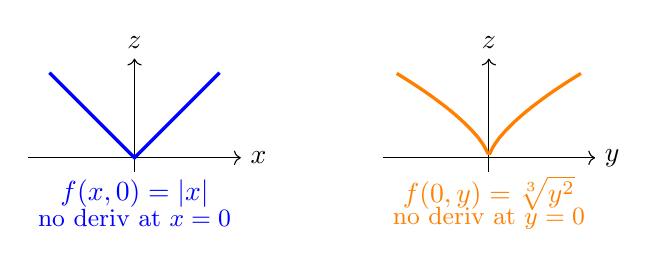
\begin{tikzpicture}[scale=0.9]
  \begin{scope}[xshift=0cm]
    \draw[->] (-1.5,0)--(1.5,0) node[right]{$x$};
    \draw[->] (0,-0.2)--(0,1.4) node[above]{$z$};
    \draw[blue, very thick] (-1.2,1.2) -- (0,0) -- (1.2,1.2);
    \node[blue] at (0,-0.5) {$f(x,0)=|x|$};
    \node[blue] at (0,-0.85) {\small no deriv at $x=0$};
  \end{scope}
  \begin{scope}[xshift=5cm]
    \draw[->] (-1.5,0)--(1.5,0) node[right]{$y$};
    \draw[->] (0,-0.2)--(0,1.4) node[above]{$z$};
    \draw[orange, very thick, domain=-1.3:1.3, samples=80]
      plot (\x, {abs(\x)^(2/3)});
    \node[orange] at (0,-0.5) {$f(0,y)=\sqrt[3]{y^2}$};
    \node[orange] at (0,-0.85) {\small no deriv at $y=0$};
  \end{scope}
\end{tikzpicture}
\end{center}
$f$ is continuous at $(0,0)$ but $f'_x(0,0)$ and $f'_y(0,0)$ do \textbf{not exist}.
\end{example}

\begin{example}[Differentiable, but partials NOT continuous]
\[
  f(x,y)=\begin{cases}
    (x^2+y^2)\sin\dfrac{1}{x^2+y^2},&(x,y)\ne(0,0),\\0,&(x,y)=(0,0).
  \end{cases}
\]
\textbf{Continuous at $(0,0)$}: $|f|\le\rho^2\to 0$.\\[4pt]
\textbf{Partial derivatives at $(0,0)$}: $f'_x(0,0)=\lim_{\Delta x\to 0}\Delta x\sin\dfrac{1}{(\Delta x)^2}=0$.
Similarly $f'_y(0,0)=0$.\\[4pt]
\textbf{Differentiability check}:
\[
  \varepsilon = \frac{\Delta f - 0\cdot\Delta x - 0\cdot\Delta y}{\Delta\rho}
  = \frac{(\Delta\rho)^2\sin\frac{1}{(\Delta\rho)^2}}{\Delta\rho}
  = \Delta\rho\cdot\underbrace{\sin\frac{1}{(\Delta\rho)^2}}_{\text{bounded}} \to 0.
\]
So $f$ \textbf{is differentiable} at $(0,0)$.\\[4pt]
\textbf{Partials not continuous}: For $(x,y)\ne(0,0)$:
\[
  f'_x(x,y) = 2x\sin\tfrac{1}{x^2+y^2} - \tfrac{2x}{x^2+y^2}\cos\tfrac{1}{x^2+y^2}.
\]
Along $y=0$, $x\to 0$: second term $\sim \frac{2}{x}\cos\frac{1}{x^2}$ is unbounded.
Hence $f'_x$ is \textbf{not continuous} at $(0,0)$.
\end{example}

%----------------------------------------------------------
\section*{Geometric Interpretation of the Differential}
%----------------------------------------------------------

\begin{center}
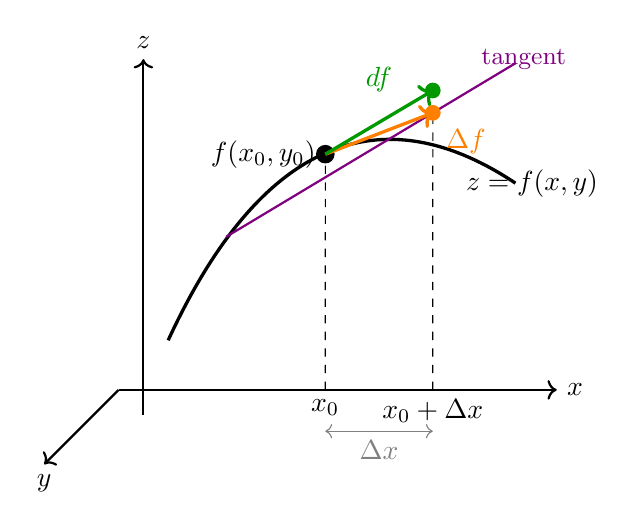
\begin{tikzpicture}[scale=1.05]
  % Axes
  \draw[->, thick] (-0.3,0) -- (5.0,0) node[right] {$x$};
  \draw[->, thick] (0,-0.3) -- (0,4.0) node[above] {$z$};
  \draw[->, thick] (-0.3,0) -- (-1.2,-0.9) node[below] {$y$};

  % Surface curve (cross-section)
  \draw[black, very thick] (0.3,0.6) .. controls (1.5,3.2) and (3.0,3.5) .. (4.5,2.5);
  \node at (4.7,2.5) {$z=f(x,y)$};

  % Base point
  \coordinate (P) at (2.2,2.85);
  \coordinate (Q) at (3.5,3.35);  % actual point after increment
  \coordinate (R) at (3.5,3.62);  % tangent plane point

  \filldraw[black] (P) circle (3pt) node[left] {$f(x_0,y_0)$};

  % x0, x0+Dx markers on axis
  \draw[dashed] (2.2,0) node[below] {$x_0$} -- (P);
  \draw[dashed] (3.5,0) node[below] {$x_0+\Delta x$} -- (Q);

  % Tangent line (purple)
  \draw[violet, thick] (1.0,1.85) -- (4.5,3.95);
  \node[violet] at (4.6,4.0) {\small tangent};

  % Actual increment Df (orange)
  \draw[orange, very thick, ->] (P) -- (Q);
  \node[orange] at (3.9,3.0) {$\Delta f$};

  % Differential df (green)
  \draw[green!60!black, very thick, ->] (P) -- (R);
  \node[green!60!black] at (2.85,3.75) {$df$};

  % horizontal bracket
  \draw[<->, gray] (2.2,-0.5) -- (3.5,-0.5) node[midway, below] {$\Delta x$};

  \filldraw[orange] (Q) circle (2.5pt);
  \filldraw[green!60!black] (R) circle (2.5pt);
\end{tikzpicture}
\end{center}

\[
  \Delta f(x_0,y_0) = f(x_0+\Delta x,\,y_0+\Delta y)-f(x_0,y_0)
  \quad\text{(actual increment, orange)}
\]
\[
  df(x_0,y_0) = f'_x(x_0,y_0)\,\Delta x + f'_y(x_0,y_0)\,\Delta y
  \quad\text{(linear approximation along tangent plane, green)}
\]

\subsection*{Tangent Plane}

The \textbf{tangent plane} to $z=f(x,y)$ at $(x_0,y_0,z_0)$ where $z_0=f(x_0,y_0)$:
\[
  \boxed{z - z_0 = f'_x(x_0,y_0)\,(x-x_0) + f'_y(x_0,y_0)\,(y-y_0)}
\]

\end{document}
